\documentclass[11pt]{article}

% This file will be kept up-to-date at the following GitHub repository:
%
% https://github.com/automl-conf/LatexTemplate
%
% Please file any issues/bug reports, etc. you may have at:
%
% https://github.com/automl-conf/LatexTemplate/issues

\usepackage{microtype} % microtypography
\usepackage{booktabs}  % tables
\usepackage{url}  % urls

% AMS math
\usepackage{amsmath}
\usepackage{amsthm}

% With no package options, the submission will be anonymized, the supplemental
% material will be suppressed, and line numbers will be added to the manuscript.
%
% To hide the supplementary material (e.g., for the first submission deadline),
% use the [hidesupplement] option:
%
% \usepackage[hidesupplement]{automl}
%
% To compile a non-anonymized camera-ready version, add the [final] option (for
% the main track), or the [finalworkshop] option (for the workshop track), e.g.,
%
% \usepackage[final]{automl}
% \usepackage[finalworkshop]{automl}
%
% or
%
% \usepackage[final, hidesupplement]{automl}
% \usepackage[finalworkshop, hidesupplement]{automl}

\usepackage[final]{automl}

% You may use any reference style as long as you are consistent throughout the
% document. As a default we suggest author--year citations; for bibtex and
% natbib you may use:

\usepackage{natbib}
\bibliographystyle{apalike}

% and for biber and biblatex you may use:

% \usepackage[%
%   backend=biber,
%   style=authoryear-comp,
%   sortcites=true,
%   natbib=true,
%   giveninits=true,
%   maxcitenames=2,
%   doi=false,
%   url=true,
%   isbn=false,
%   dashed=false
% ]{biblatex}
% \addbibresource{...}

% Own packages
\usepackage{hyperref}
\hypersetup{
    colorlinks=true,
    linkcolor=black,
    filecolor=black,      
    urlcolor=black,
    pdftitle={Overleaf Example},
    pdfpagemode=FullScreen,
    }
\usepackage{float}
\usepackage{adjustbox}
\usepackage{longtable}
\usepackage{tabularx}
\usepackage{caption}
\usepackage{rotating}

\title{AutoML project: Tuning a majority voting ensemble consisting of random forest classifier, gradient boosting classifier and SVM classifier using DEHB}

% The syntax for adding an author is
%
% \author[i]{\nameemail{author name}{author email}}
%
% where i is an affiliation counter. Authors may have
% multiple affiliations; e.g.:
%
% \author[1,2]{\nameemail{Anonymous}{anonymous@example.com}}

\author[1]{\nameemail{Constantin von Crailsheim}{C.Crailsheim@campus.lmu.de}}

% the list might continue:
% \author[2,3]{\nameemail{Author 2}{email2@example.com}}
% \author[3]{\nameemail{Author 3}{email3@example.com}}
% \author[4]{\nameemail{Author 4}{email4@example.com}}

% if you need to force a linebreak in the author list, prepend an \author entry
% with \\:

% \author[3]{\\\nameemail{Author 5}{email5@example.com}}

% Specify corresponding affiliations after authors, referring to counter used in
% \author:

\affil[1]{LMU Munich, Institute of Statistics}

% the list might continue:
% \affil[2]{Institution 2}
% \affil[3]{Institution 3}
% \affil[4]{Institution 4}

% define PDF metadata, please fill in to aid in accessibility of the resulting PDF
\hypersetup{%
  pdfauthor={}, % will be reset to "Anonymous" unless the "final" package option is given
  pdftitle={},
  pdfsubject={},
  pdfkeywords={}
}

\begin{document}

\maketitle

\begin{abstract}
The AutoML system tunes a ML pipeline consisting of an imputer, an optional sampler, an optional scaler and a choice of three models. Since the tasks are imbalanced tabular datasets, a random forest classifier, a gradient boosting classifier and a SVM classifier are reasonable choices, which should yield a good overall prediction by majority voting. I used DEHB as an optimizer, which combines the advantages of differential evolutions and hyperband, i.e., generating promising new hyperparameter configurations for more costly evaluations based on initial cheap evaluations. Overall, the improvement in performance compared to the untuned random forest classifier baseline is 0.8\% and 25.9\% as measured by balanced accuarcy. Thus the AutoML system outperforms the baseline across all datasets and the algorithm is significantly different for 9 out of 10 datasets by the McNemar test. The source code is available at: \url{https://github.com/constantin-crailsheim/automl_imbalanced}
\end{abstract}

% content will be automatically hidden during submission
% \begin{acknowledgements}

% \end{acknowledgements}

\section{Introduction}

The objective of the AutoML system is to yield good performance as measured by the balanced accuracy on imbalanced tabular datasets and to be able to deal with missing values. Thus, it optimizes a ML pipeline consisting of five elements. First, a choice of two imputers replaces missing values. Then, an optional sampling method is applied to deal with imbalance in the targets, which can be under- and/or oversampling methods. Next, the pre-processed integer features are rounded such that they do not take values that would not appear in the original data. After optionally normalizing all features, three different models were fitted, i.e., a random forest classifier, a gradient boosting classifier and a SVM classifier. The pre-processing choices and the hyperparameters of the model were optimized by DEHB, which is a computationally cheap optimizer that works well on discrete search spaces. The final predictions are derived by majority voting over the individual predictions of the best pipelines for each model. This means that the overall predictions should be in particular good if the errors of the models are not too correlated.

\section{Method}

This section outlines the specific choices of the AutoML system and how it will be optimized and evaluated. The choices of \texttt{sklearn.impute} for the imputation strategy are:
\begin{itemize}
\item The \href{https://scikit-learn.org/stable/modules/generated/sklearn.impute.SimpleImputer.html}{\texttt{SimpleImputer}} is an univariate imputer, which completes missing values with a descriptive statistic per feature. I chose the median, since it is less sensitive to outliers than the mean.
\item The \href{https://scikit-learn.org/stable/modules/generated/sklearn.impute.KNNImputer.html#sklearn.impute.KNNImputer}{\texttt{KNNImputer}} replaces missing values by the mean value of its 5 nearest neighbors as default based on Euclidian distance of their non-missing observations of the same feature. 
\end{itemize}

The choices of \texttt{imblearn} for the data-level sampling method to yield a balanced dataset are:
\begin{itemize}
\item \href{https://imbalanced-learn.org/stable/references/generated/imblearn.over_sampling.SMOTE.html}{\texttt{SMOTE}} as an oversampling approach generates new samples of the minority class by interpolating between existing observations of the minority class, where no distinction is made between easy and hard samples. 
\item \href{https://imbalanced-learn.org/stable/references/generated/imblearn.under_sampling.TomekLinks.html}{\texttt{TomekLinks}} as an undersampling approach removes samples from the majority class, if they are nearest neighbors to a minority class sample, thus removing noisy borderline samples of the majority class. 
\item \href{https://imbalanced-learn.org/stable/references/generated/imblearn.combine.SMOTETomek.html}{\texttt{SMOTETomek}} combines SMOTE and Tomek links.
\item No sampling method would allow algorithmic-level methods to deal with the imbalanced data. 
\end{itemize}

The above pre-processing methods could generate numeric values for features that should contain only integers (e.g., ordinal categorical features), since they impute missing values by means or medians and generate new samples by interpolation. Thus, I added another layer to the pipeline, which rounds all observations of these features to the closest integer. \\

The last step of pre-processing is  the choice of whether to apply the \href{https://scikit-learn.org/stable/modules/generated/sklearn.preprocessing.StandardScaler.html}{\texttt{StandardScaler}} of \texttt{sklearn.preprocessing} to standardize the features. This will be in particular useful for the SVM, since an RBF kernel assumes features centered around zero and similar variance across features. \\

Subsequently, the hyperparameters of the three models of the ensemble were optimized, where I defined the search space with the \href{https://automl.github.io/ConfigSpace/main/}{\texttt{ConfigSpace}} package. For almost all hyperparameters, the default was set to the default specified for each model. I chose the search space mostly such that it is centered around the default while accounting for log scale. In those cases where the default would be a the lower end of a reasonable search space, I chose the upper bound reasonably higher. \\

The first model in the ensemble is a \href{https://scikit-learn.org/stable/modules/generated/sklearn.ensemble.RandomForestClassifier.html}{\texttt{RandomForestClassifier}} from \texttt{sklearn.ensemble}. It can handle all data types well and generalizes well by having a low variance due to ensembling over relatively uncorrelated models. The hyperparameters, which will all be sampled uniformly, are:

\begin{table}[H]
\centering
\begin{tabular}{ | c | c | c | c | c | c | }
 \hline
  Hyperparameter & Data type & Search space & Default & Other \\
 \hline
 \texttt{criterion} & Categorical & \{\texttt{gini}, \texttt{entropy}, \texttt{log\_loss}\} & \texttt{gini} &   \\ 
 \texttt{max\_depth}  & Integer & [5,15] & 10 &  \\ 
 \texttt{min\_samples\_split} & Integer & [1, 32] & 2 & Log scale \\ 
 \texttt{min\_samples\_leaf} & Integer & [1, 16] & 1 & Log scale  \\ 
 \texttt{max\_features} & Integer & [0.1, 0.9] & 0.5 &   \\  
 \texttt{class\_weight} & Categorical & \{\texttt{balanced}, \texttt{balanced\_subsample}, \texttt{None}\}  & \texttt{None} &  \\ 
 \hline
\end{tabular}
\end{table}

The \texttt{class\_weight} is an algorithm-level method that deals with imbalanced data by giving less frequent classes more weight. It will only have an effect if no data-level sampling method was used, since in the other case the dataset passed to the model will be balanced. \\

The second model in the ensemble is a \href{https://scikit-learn.org/stable/modules/generated/sklearn.ensemble.GradientBoostingClassifier.html}{\texttt{GradientBoostingClassifier}} from \texttt{sklearn.ensemble}. It has strong predictive performance by iteratively fitting weak learners on the error of the previous learner and has similar advantages as the \texttt{RandomForestClassifier}. The hyperparameters are:

\begin{table}[H]
\centering
\begin{tabular}{ | c | c | c | c | c | c | }
 \hline
  Hyperparameter & Data type & Search space & Default & Other \\
 \hline
 \texttt{loss} & Categorical & \{\texttt{log\_loss}, \texttt{exponential}\} & \texttt{log\_loss} &  \\ 
 \texttt{learning\_rate} & Float & [0.01, 1] & 0.1 & Log scale  \\ 
 \texttt{criterion} & Categorical & \{\texttt{friedman\_mse}, \texttt{squared\_error}\} & \texttt{friedman\_mse} &   \\ 
 \texttt{min\_samples\_split} & Integer & [1, 32] & 2 & Log scale \\ 
 \texttt{min\_samples\_leaf} & Integer & [1, 16] & 1 & Log scale  \\
 \texttt{max\_depth}  & Integer & [2,10] & 3 &  \\ 
 \hline
\end{tabular}
\end{table}

\newpage
The third model in the ensemble is a Support Vector Classifier (\href{https://scikit-learn.org/stable/modules/generated/sklearn.svm.SVC.html#sklearn.svm.SVC}{\texttt{SVC}}) from \texttt{sklearn.svm}. This model works in particular well on easily to separate datasets, on small datasets and in high-dimensional spaces \citep{GfG}. The hyperparameters are:

\vspace{-0.3cm}
\begin{table}[H]
\centering
\begin{tabular}{ | c | c | c | c | c | c | }
 \hline
  Hyperparameter & Data type & Search space & Default & Other \\
 \hline
 \texttt{C} & Float & [0.1, 10]  & 1.0 & Log scale \\ 
 \texttt{kerne}l & Categorical & \{\texttt{linear}, \texttt{poly}, \texttt{rbf}, \texttt{sigmoid}\}  & \texttt{rbf} &   \\ 
 \texttt{shrinking} & Boolean & \{\texttt{True}, \texttt{False}\} & True &  \\ 
 \texttt{to}l & Float & [1e-4,1e-2] & 1e-3 &  \\ 
 \texttt{class\_weight} & Categorical & \{\texttt{balanced}, \texttt{None}\}  & \texttt{None} &  \\ 
 \hline
\end{tabular}
\end{table}
\vspace{-0.3cm}

To optimize the hyperparameter of the AutoML system, I used \href{https://github.com/automl/dehb}{\texttt{DEHB}} by \citet{dehb}, which combines differential evolution and hyperband. Differential evolution constructs a new mutant vector from three random parents and then generates the offspring by randomly selecting values from the new mutant vector with probability $p$ and otherwise from one of the corresponding parents. Hyperband allows to search the whole search space with cheap evaluations and only trains more costly models on promising areas of the search space. The algorithm starts by sampling $N$ random hyperparameter configurations, which are evaluated at the lowest budget. Then the best $1/\eta$ of these configurations are evaluated at a $\eta$-times higher budget and this process is repeated until the highest fidelity (denoted here by $f$) is reached, thus $N=\eta^{f-1}$. After completing one iteration, the algorithm restarts with new instantiations and evaluates these at the second lowest fidelity, thereby hedging against bad initializations. \texttt{DEHB} combines both approaches by generating the hyperparameter configurations for the next fidelity by differential evolution from the lower fidelity as parent pool. The authors state that \texttt{DEHB} is computationally cheap with high speed-up gains compared to \texttt{BOHB}. Furthermore, it has strong final performance for discrete search spaces, which I have for various hyperparameters. The authors experiments have shown that \texttt{DEHB} also outperforms \texttt{SMAC} by mean ranks across all of their chosen benchmarks. For those reasons, I chose DEHB as an efficient optimizer for this problem. \\

For the optimization, I set $\eta=3$ and $f=4$, which implies an initial population of $N=3^{3}=27$. I set the budget for the \texttt{RandomForestClassifier} and the \texttt{GradientBoostingClassifier}, as indicated by the number of trees in the forest, to a minimum of 10 and maximum of 270. For \texttt{SVC}, I chose the maximum number of iterations as budget and I set it to a minimum of 500 and maximum of 13500. However, the runtime between the lowest and largest budget usually did not differ too much since the SVM optimizer most likely already converged in most cases and the evaluation was relatively cheap compared to the forest based classifiers for most datasets. Thus, the \texttt{SVC} mostly benefits from differential evolution and the successive halving element is not as important, since many configurations can be tested irrespecitively. Hence, I allocated 40\% of the maximum cost to optimizing the forest based models and 20\% to optimizing the \texttt{SVC}. \\

To evaluate the performance of the AutoML system, I used 3-fold external and 4-fold internal cross-validation. I used stratified CV to ensure that the class imbalance of the targets is preserved in each fold. Given a total budget of 3600 seconds per dataset, a total of 1200 second could be used to optimize the AutoML system in each fold. Since the budget is not that larger after accounting for cross-validation, I tuned only a selection of hyperparameters of the actual model and the hyperparameters of the preprocessing functions were kept at their default values. \\

After the optimization routine, all three model pipelines are passed to the \href{https://scikit-learn.org/stable/modules/generated/sklearn.ensemble.VotingClassifier.html}{\texttt{VotingClassifier}} from \texttt{sklearn.ensemble} and fitted with their incumbent configurations. Then the imbalance sampling is removed from the pipeline to not sample for the test set. Thus, the final AutoML system is an ensemble of three pipelines with majority voting for the final classification. 

\section{Experiments}

To run the optimization, I used a M1 Pro chip and 32 GB RAM from 2021. The external cross-validation performance in terms of balanced accuracy of the AutoML system vs. the untuned \texttt{RandomForestClassifer} baseline for each dataset id is shown below:

\vspace{-0.2cm}
\begin{table}[H]
\centering
\begin{tabular}{lrrrrrrrrrr}
\toprule
Model &   976 &   980 &  1002 &  1018 &  1019 &  1021 &  1040 &  1053 &  1461 &  41160 \\
\midrule
Baseline & 0.962 & 0.939 & 0.547 & 0.554 & 0.989 & 0.932 & 0.960 & 0.594 & 0.695 & 0.571 \\
AutoML system & 0.990 & 0.982 & 0.806 & 0.809 & 0.997 & 0.957 & 0.992 & 0.657 & 0.838 & 0.743 \\
\midrule
Improvement & 0.027 & 0.043 & 0.259 & 0.254 & 0.008 & 0.025 & 0.032 & 0.063 & 0.143 & 0.172 \\
McNemar test & 37.19 & 30.94 & 927.63 & 906.28 & 8.75 & 11.40 & 1.86 & 287.88 & 660.02 & 117.14 \\
\bottomrule
\end{tabular}
\end{table}
\vspace{-0.2cm}

Hence, the AutoML system outperforms the baseline across all datasets with an improvement between 0.8\% and 25.9\%. To evaluate whether the two algorithms are significantly different, I used the McNemar test, which was computed over the concatenated predictions of all folds. The reference distribution is $\chi_{1}^{2}$ and thus the algorithms would be significantly different at the 5\%-level if the test statistic is larger than 3.84, which is the case for all datasets except for dataset 1040. However, for this dataset the balanced accuracy is still 3.2\% better and above 99\%. \\

The plots of the trajectories for each dataset are shown in appendix A. For dataset 976, 980 1019, the \texttt{SVC} is the top performing estimator, followed by the \texttt{GradientBoostingClassifier} and the \texttt{RandomForestClassifier}. For the other datasets, the ranking is not as clear. For the last two datasets, the \texttt{SVC} has the worst performance, most likely since SVMs are costlier to fit given the large number of observations and less iterations to tune the hyperparameters were possible. However, the overall performance of the AutoML system is still similar to the best individual pipelines due to majority voting. The benchmarks are usually outperformed after at most 50 seconds, except for the last two datasets due to the underperforming \texttt{SVC}. The final externally cross-validated performance is a bit lower than the performances of the individual algorithms for a few datasets, since the performance of the individual algorithms tends to be overly optimistic due to the hyperparameters being tuned on that specific fold. \\

The chosen incumbents for each model pipeline for all datasets are shown in appendix B. Some key trends are as following: The preferred sampling method for \texttt{RandomForestClassifier} and \texttt{SVC} is quite mixed, but for the \texttt{GradientBoostingClassifier} only oversampling or mixed methods were selected. As expected, \texttt{SVC} uses the \texttt{StandardScaler} for all datasets, except 1019. If no sampling method was chosen, the imbalance was always accounted for by class weights. Lastly, the \texttt{RandomForestClassifier} prefers on average deeper trees than the \texttt{GradientBoostingClassifier}. \\

\section{Conclusion}

The AutoML system outperforms the benchmark across all datasets and has thus has proven to be useful. However, some improvements are still possible if a larger budget would be available. The hyperparameters of the pre-processing methods could be also tuned to fit better to each dataset and algorithm. Furthermore, a stacking classifier could be trained on the three algorithms, which would allow to find the best weighted combination of the predictions of each individual algorithm for the final prediction of the AutoML system. I conducted experiments with stacking, but the training on the final incumbents with the highest budgets took fairly long, thus I decided to use the budget rather to improve the performance of the individual estimators. Overall, however, this AutoML system is capable of tuning well performing pipelines for imbalanced classification tasks.


\bibliography{References.bib}

% supplemental material -- everything hereafter will be suppressed during
% submission time if the hidesupplement option is provided!

\newpage
\appendix

\section{Trajectories}

The following plots show the trajectories of the incumbent performance of all three model pipelines (\texttt{RandomForestClassifier} (RFC), \texttt{RandomForestClassifier} (GBC), \texttt{SVC}) evaluated with internal CV in each fold, over runtime. Furthermore, the external CV of the untuned RFC baseline is plotted as grey horizontal line and the external CV of the final performance of the AutoML system is plotted as purple dot at the maximum runtime per model in each fold.

\begin{figure}[H]
 \centering
  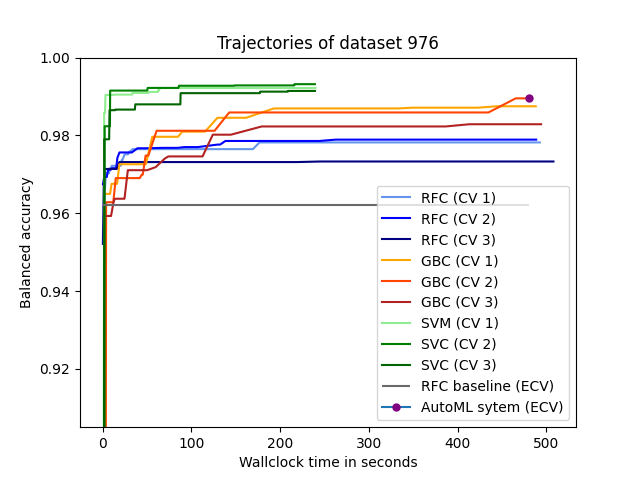
\includegraphics[width=0.75\textwidth]{fig/plot_dataset_976.png}
  \caption{Trajectories for dataset 976 with 9961 observations and 14 features.}
\end{figure}

\begin{figure}[H]
 \centering
  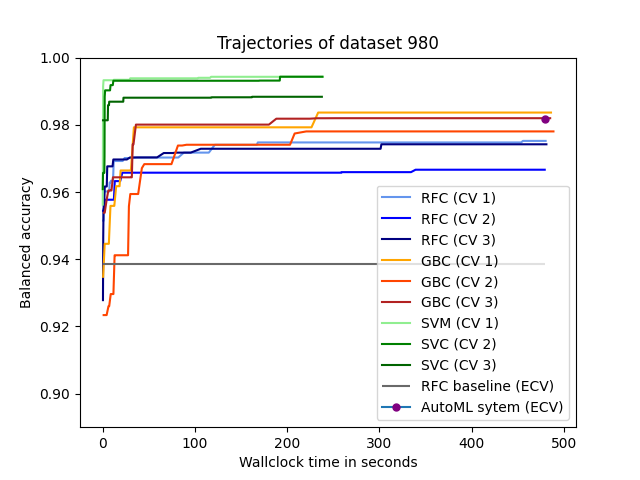
\includegraphics[width=0.75\textwidth]{fig/plot_dataset_980.png}
  \caption{Trajectories for dataset 980 with 5620 observations and 64 features.}
\end{figure}

\begin{figure}[H]
 \centering
  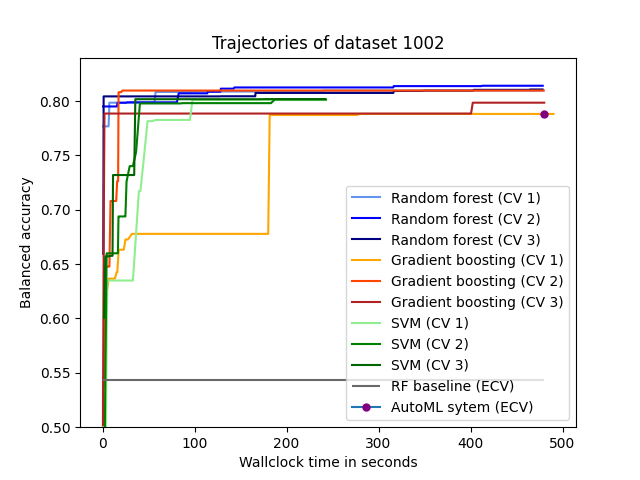
\includegraphics[width=0.75\textwidth]{fig/plot_dataset_1002.png}
  \caption{Trajectories for dataset 1002 with 7485 observations and 55 features.}
\end{figure}

\begin{figure}[H]
 \centering
  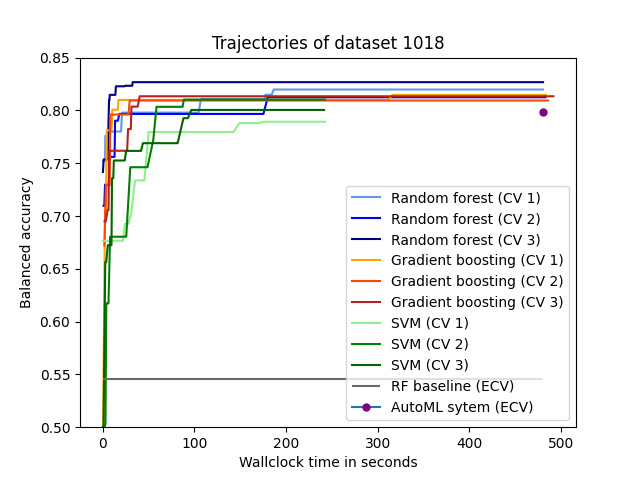
\includegraphics[width=0.75\textwidth]{fig/plot_dataset_1018.png}
  \caption{Trajectories for dataset 1018 with 8844 observations and 56 features.}
\end{figure}

\begin{figure}[H]
 \centering
  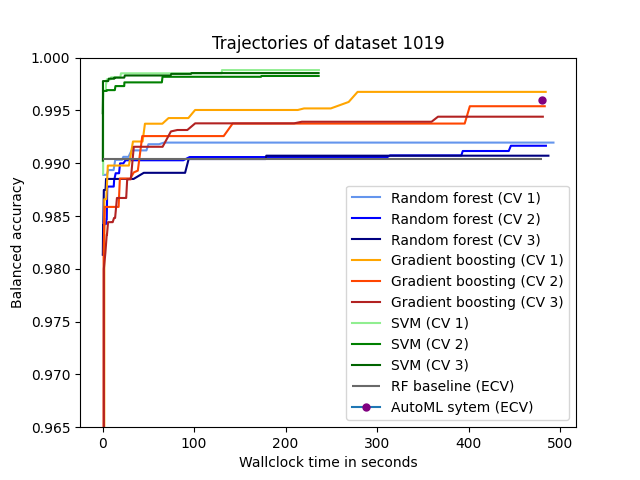
\includegraphics[width=0.75\textwidth]{fig/plot_dataset_1019.png}
  \caption{Trajectories for dataset 1019 with 10992 observations with 16 features}
\end{figure}

\begin{figure}[H]
 \centering
  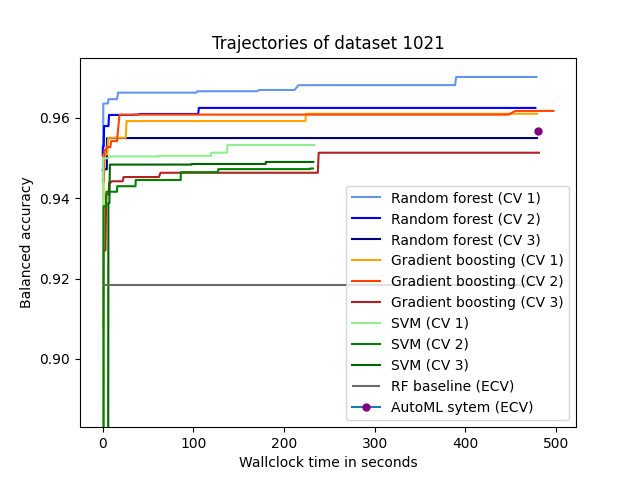
\includegraphics[width=0.75\textwidth]{fig/plot_dataset_1021.png}
  \caption{Trajectories for dataset 1021 with 5473 observations and 10 features.}
\end{figure}

\begin{figure}[H]
 \centering
  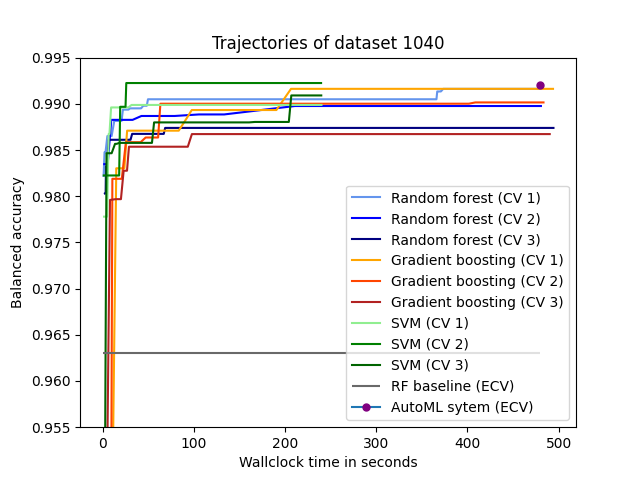
\includegraphics[width=0.75\textwidth]{fig/plot_dataset_1040.png}
  \caption{Trajectories for dataset 1040 with 14395 observations and 108 features.}
\end{figure}

\begin{figure}[H]
 \centering
  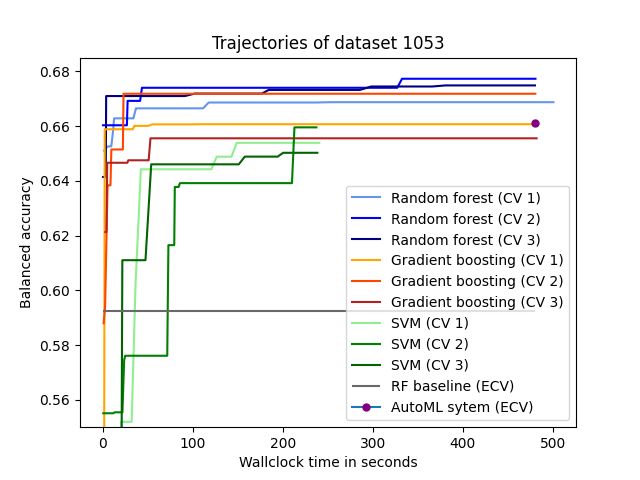
\includegraphics[width=0.75\textwidth]{fig/plot_dataset_1053.png}
  \caption{Trajectories for dataset 1053 with 10885 observations and 21 features.}
\end{figure}

\begin{figure}[H]
 \centering
  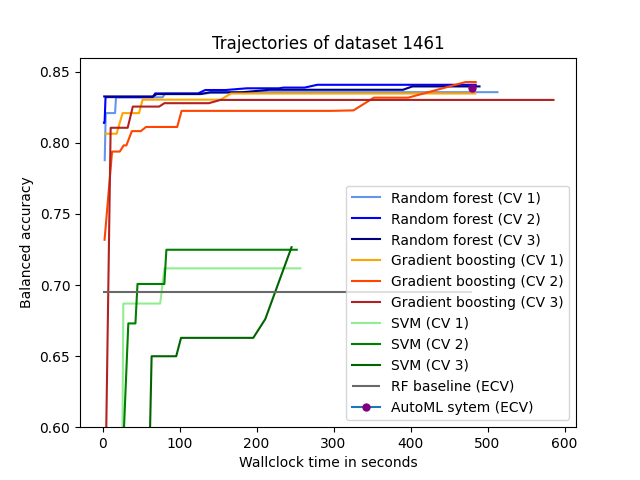
\includegraphics[width=0.75\textwidth]{fig/plot_dataset_1461.png}
  \caption{Trajectories for dataset 1461 with 45221 observations and 16 features.}
\end{figure}

\begin{figure}[H]
 \centering
  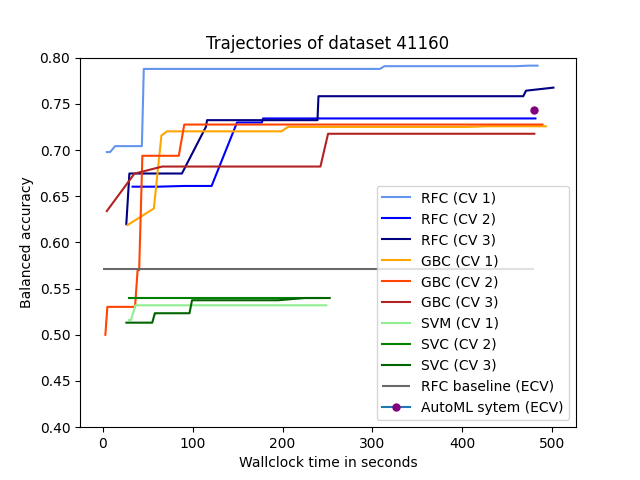
\includegraphics[width=0.75\textwidth]{fig/plot_dataset_41160.png}
  \caption{Trajectories for dataset 41660 with 31406 observations and 22 features.}
\end{figure}

\section{Incumbent hyperparameters}

The following tables shows the incumbent hyperparameter configurations for each algorithm and each dataset in each fold. 

\begin{sidewaystable}
\footnotesize
\caption{Incumbent hyperparameters configurations for the random forest classifier}
\center
\begin{tabularx}{22cm}{lllllllXXXX}
\toprule
Dataset ID & CV fold & Imputer & Sampler & Scaler & Criterion & Max depth & Min samples per split & Min samples per leaf & Max features & Class weight \\
\midrule
976 & 1 & Simple & SMOTETomek & True & entropy & 19 & 6 & 1 & 0.527 & balanced\_subsample \\
976 & 2 & Simple & SMOTETomek & True & log\_loss & 25 & 1 & 1 & 0.419 & balanced\_subsample \\
976 & 3 & Simple & SMOTE & False & entropy & 18 & 4 & 2 & 0.676 & balanced \\
\midrule
980 & 1 & KNN & SMOTE & False & entropy & 22 & 4 & 8 & 0.190 & balanced\_subsample \\
980 & 2 & Simple & SMOTE & True & entropy & 7 & 9 & 8 & 0.202 & balanced\_subsample \\
980 & 3 & Simple & SMOTE & True & entropy & 7 & 2 & 3 & 0.357 & balanced \\
\midrule
1002 & 1 & KNN & Tomek & True & entropy & 5 & 4 & 5 & 0.152 & balanced \\
1002 & 2 & KNN & SMOTE & True & entropy & 6 & 13 & 1 & 0.106 & None \\
1002 & 3 & Simple & None & True & entropy & 5 & 8 & 6 & 0.262 & balanced \\
\midrule
1018 & 1 & KNN & Tomek & False & gini & 5 & 10 & 1 & 0.188 & balanced\_subsample \\
1018 & 2 & KNN & None & False & entropy & 6 & 24 & 4 & 0.116 & balanced \\
1018 & 3 & Simple & Tomek & True & entropy & 5 & 2 & 9 & 0.127 & balanced\_subsample \\
\midrule
1019 & 1 & KNN & SMOTETomek & True & entropy & 17 & 4 & 2 & 0.664 & balanced\_subsample \\
1019 & 2 & Simple & SMOTETomek & True & log\_loss & 21 & 3 & 3 & 0.295 & None \\
1019 & 3 & Simple & SMOTETomek & False & entropy & 20 & 3 & 6 & 0.464 & balanced \\
\midrule
1021 & 1 & KNN & SMOTETomek & True & gini & 13 & 2 & 7 & 0.203 & balanced \\
1021 & 2 & Simple & SMOTETomek & False & gini & 9 & 4 & 5 & 0.416 & balanced \\
1021 & 3 & KNN & SMOTE & False & entropy & 14 & 4 & 9 & 0.568 & balanced \\
\midrule
1040 & 1 & KNN & Tomek & True & log\_loss & 12 & 1 & 15 & 0.513 & balanced \\
1040 & 2 & KNN & SMOTE & True & log\_loss & 6 & 32 & 3 & 0.285 & balanced\_subsample \\
1040 & 3 & Simple & None & True & log\_loss & 17 & 1 & 5 & 0.365 & balanced\_subsample \\
\midrule
1053 & 1 & KNN & Tomek & False & log\_loss & 8 & 10 & 16 & 0.590 & balanced\_subsample \\
1053 & 2 & Simple & Tomek & True & gini & 12 & 24 & 4 & 0.400 & balanced \\
1053 & 3 & KNN & Tomek & False & entropy & 25 & 9 & 14 & 0.555 & balanced \\
\midrule
1461 & 1 & Simple & None & False & entropy & 11 & 5 & 16 & 0.628 & balanced \\
1461 & 2 & Simple & None & False & gini & 9 & 10 & 1 & 0.390 & balanced \\
1461 & 3 & KNN & Tomek & False & entropy & 15 & 8 & 15 & 0.765 & balanced\_subsample \\
\midrule
41160 & 1 & Simple & Tomek & False & log\_loss & 12 & 28 & 11 & 0.811 & balanced \\
41160 & 2 & Simple & Tomek & False & gini & 10 & 3 & 5 & 0.379 & balanced \\
41160 & 3 & KNN & None & True & gini & 12 & 5 & 9 & 0.851 & balanced \\
\bottomrule
\end{tabularx}
\end{sidewaystable}


\begin{sidewaystable}
\footnotesize
\caption{Incumbent hyperparameters configurations for the gradient boosting classifier}
\center
\begin{tabular}{lllllllllll}
\toprule
Dataset ID & CV fold & Imputer & Sampler & Scaler & Loss & Learning rate & Criterion & Min samples per split & Min samples per leaf & Max depth \\
\midrule
976 & 1 & Simple & SMOTE & False & exponential & 0.603 & squared\_error & 2 & 7 & 6 \\
976 & 2 & Simple & SMOTETomek & True & log\_loss & 0.522 & squared\_error & 23 & 3 & 5 \\
976 & 3 & Simple & SMOTETomek & True & exponential & 0.815 & squared\_error & 5 & 3 & 3 \\
\midrule
980 & 1 & Simple & SMOTE & True & log\_loss & 0.598 & squared\_error & 7 & 4 & 4 \\
980 & 2 & KNN & SMOTETomek & True & log\_loss & 0.432 & friedman\_mse & 9 & 7 & 3 \\
980 & 3 & Simple & SMOTETomek & True & exponential & 0.322 & squared\_error & 6 & 1 & 5 \\
\midrule
1002 & 1 & KNN & SMOTETomek & True & log\_loss & 0.010 & squared\_error & 3 & 7 & 2 \\
1002 & 2 & KNN & SMOTETomek & False & log\_loss & 0.013 & squared\_error & 7 & 6 & 2 \\
1002 & 3 & KNN & SMOTE & True & exponential & 0.021 & friedman\_mse & 12 & 7 & 4 \\
\midrule
1018 & 1 & KNN & SMOTETomek & True & log\_loss & 0.061 & friedman\_mse & 6 & 1 & 3 \\
1018 & 2 & Simple & SMOTETomek & True & log\_loss & 0.185 & squared\_error & 6 & 12 & 3 \\
1018 & 3 & KNN & SMOTE & True & exponential & 0.054 & friedman\_mse & 2 & 1 & 3 \\
\midrule
1019 & 1 & Simple & SMOTE & True & exponential & 0.398 & squared\_error & 31 & 4 & 4 \\
1019 & 2 & Simple & SMOTETomek & True & log\_loss & 0.158 & friedman\_mse & 7 & 1 & 3 \\
1019 & 3 & Simple & SMOTE & False & exponential & 0.666 & friedman\_mse & 5 & 6 & 4 \\
\midrule
1021 & 1 & KNN & SMOTETomek & True & exponential & 0.018 & friedman\_mse & 7 & 6 & 5 \\
1021 & 2 & Simple & SMOTE & False & log\_loss & 0.034 & squared\_error & 3 & 4 & 5 \\
1021 & 3 & KNN & SMOTETomek & True & log\_loss & 0.141 & friedman\_mse & 7 & 3 & 6 \\
\midrule
1040 & 1 & KNN & SMOTETomek & True & log\_loss & 0.048 & friedman\_mse & 5 & 3 & 4 \\
1040 & 2 & Simple & SMOTE & False & exponential & 0.588 & friedman\_mse & 4 & 3 & 3 \\
1040 & 3 & Simple & SMOTE & False & log\_loss & 0.410 & friedman\_mse & 20 & 7 & 3 \\
\midrule
1053 & 1 & KNN & SMOTETomek & True & exponential & 0.014 & squared\_error & 15 & 1 & 3 \\
1053 & 2 & Simple & SMOTETomek & False & exponential & 0.021 & squared\_error & 7 & 3 & 3 \\
1053 & 3 & KNN & SMOTETomek & True & log\_loss & 0.270 & squared\_error & 8 & 8 & 2 \\
\midrule
1461 & 1 & KNN & SMOTETomek & False & exponential & 0.092 & squared\_error & 7 & 4 & 7 \\
1461 & 2 & KNN & SMOTETomek & False & log\_loss & 0.035 & friedman\_mse & 4 & 7 & 5 \\
1461 & 3 & Simple & SMOTETomek & False & log\_loss & 0.111 & friedman\_mse & 8 & 5 & 8 \\
\midrule
41160 & 1 & Simple & SMOTE & False & log\_loss & 0.023 & friedman\_mse & 16 & 2 & 11 \\
41160 & 2 & Simple & SMOTE & False & exponential & 0.043 & friedman\_mse & 30 & 2 & 9 \\
41160 & 3 & Simple & SMOTETomek & False & log\_loss & 0.058 & squared\_error & 5 & 3 & 11 \\
\bottomrule
\end{tabular}
\end{sidewaystable}

\begin{sidewaystable}
\footnotesize
\caption{Incumbent hyperparameters configurations for the SVM classifier}
\center
\begin{tabular}{llllllllll}
\toprule
Dataset ID & CV fold & Imputer & Sampler & Scaler & C & Kernel & Shrinking & Tolerance & Class weight \\
\midrule
976 & 1 & KNN & SMOTETomek & True & 8.489 & rbf & True & 0.0085 & balanced \\
976 & 2 & Simple & None & True & 8.670 & rbf & False & 0.0016 & balanced \\
976 & 3 & Simple & None & True & 4.036 & rbf & False & 0.0005 & balanced \\
\midrule
980 & 1 & Simple & SMOTETomek & True & 2.230 & poly & False & 0.0040 & balanced \\
980 & 2 & KNN & Tomek & True & 0.893 & poly & True & 0.0030 & balanced \\
980 & 3 & KNN & None & False & 1.061 & rbf & True & 0.0006 & balanced \\
\midrule
1002 & 1 & KNN & SMOTETomek & True & 0.161 & linear & True & 0.0017 & balanced \\
1002 & 2 & KNN & Tomek & True & 0.199 & linear & False & 0.0003 & balanced \\
1002 & 3 & Simple & SMOTE & True & 0.169 & linear & False & 0.0025 & balanced \\
\midrule
1018 & 1 & Simple & SMOTETomek & True & 0.213 & sigmoid & True & 0.0007 & None \\
1018 & 2 & Simple & Tomek & True & 0.621 & poly & True & 0.0001 & balanced \\
1018 & 3 & KNN & SMOTETomek & True & 0.113 & linear & True & 0.0039 & balanced \\
\midrule
1019 & 1 & Simple & None & False & 2.186 & poly & True & 0.0062 & balanced \\
1019 & 2 & Simple & SMOTETomek & False & 6.871 & rbf & True & 0.0040 & None \\
1019 & 3 & Simple & Tomek & False & 7.892 & rbf & True & 0.0003 & balanced \\
\midrule
1021 & 1 & Simple & None & True & 6.803 & rbf & True & 0.0058 & balanced \\
1021 & 2 & Simple & Tomek & True & 7.117 & rbf & True & 0.0011 & balanced \\
1021 & 3 & Simple & Tomek & True & 6.244 & rbf & True & 0.0005 & balanced \\
\midrule
1040 & 1 & KNN & SMOTE & True & 0.218 & linear & True & 0.0019 & None \\
1040 & 2 & KNN & SMOTETomek & True & 0.143 & linear & True & 0.0001 & balanced \\
1040 & 3 & KNN & SMOTE & True & 1.384 & sigmoid & False & 0.0012 & balanced \\
\midrule
1053 & 1 & Simple & None & True & 0.851 & rbf & True & 0.0009 & balanced \\
1053 & 2 & Simple & SMOTE & True & 0.384 & rbf & True & 0.0009 & balanced \\
1053 & 3 & Simple & Tomek & True & 0.900 & rbf & False & 0.0012 & balanced \\
\midrule
1461 & 1 & Simple & None & True & 0.363 & sigmoid & False & 0.0004 & balanced \\
1461 & 2 & KNN & Tomek & True & 0.399 & sigmoid & False & 0.0004 & balanced \\
1461 & 3 & Simple & SMOTETomek & True & 0.526 & rbf & False & 0.0003 & balanced \\
\midrule
41160 & 1 & Simple & SMOTETomek & True & 0.190 & sigmoid & True & 0.0002 & balanced \\
41160 & 2 & KNN & SMOTE & True & 0.586 & sigmoid & True & 0.0007 & balanced \\
41160 & 3 & KNN & SMOTETomek & True & 1.275 & rbf & False & 0.0037 & None \\
\bottomrule
\end{tabular}
\end{sidewaystable}

\section{Information about datasets}

\begin{table}[H]
\center
\caption{Meta data of each dataset}
\begin{tabular}{llllllllll}
\toprule
Dataset ID & Observations & Features & Share of underrepresented class & Total missing values \\
\midrule
976 & 9961 & 14 & 0.162 & 0 \\
980 & 5620 & 64 & 0.102 & 0 \\
1002 & 7485 & 55 & 0.106 & 0 \\
1018 & 8844 & 56 & 0.064 & 0 \\
1019 & 10992 & 16 & 0.104 & 0 \\
1021 & 5473 & 10 & 0.102 & 0 \\
1040 & 14395 & 108 & 0.062 & 0 \\
1053 & 10885 & 21 & 0.193 & 25 \\
1461 & 45211 & 16 & 0.117 & 0 \\
41160 & 31406 & 22 & 0.095 & 29756 \\
\bottomrule
\end{tabular}
\end{table}

\end{document}
